% \subsubsection{Caughey}
% ** Not in  release ** The model  is a particular case of  the Rayleigh damping
% model,   with    damping   being   proportional   only    to   the   stiffness
% matrix. Substitute with complete Rayleigh damping model for release?

\subsection{Neo-Hookean}\index{Material!Neohookean}

The Neo-Hookean constitutive law is a hyperelastic material formulation, which
results from an extension of the linear elastic relationship (Hooke's Law) for
large deformation. Thus, the model predicts nonlinear stress-strain behavior for
bodies undergoing large deformations.

\begin{figure}[!htb]
  \begin{center}
    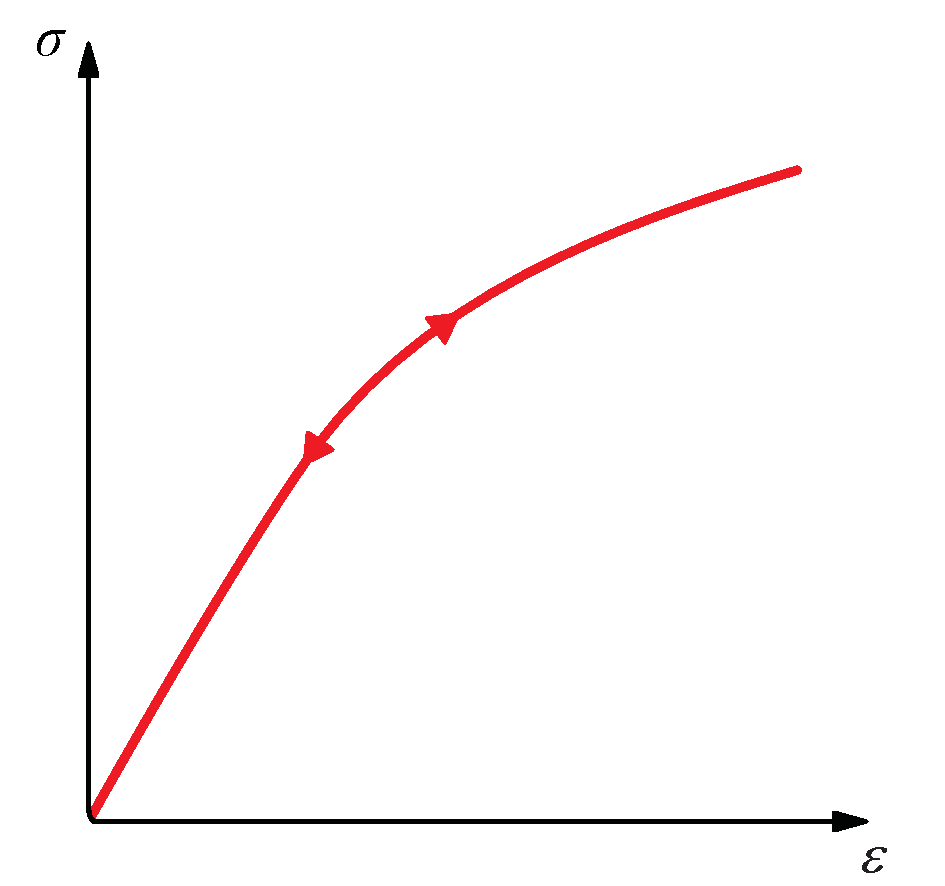
\includegraphics[width=0.4\textwidth,keepaspectratio=true]{figures/stress_strain_neo.pdf}
    \caption{Neo-hookean Stress-strain curve.}
    \label{fig:smm:cl:neo_hookean}
  \end{center}
\end{figure}

As illustrated in Figure~\ref{fig:smm:cl:neo_hookean}, the behavior is initially
linear and the mechanical behavior is very close to the corresponding linear
elastic material. This constitutive relationship, which accounts for compressibility,
 is a modified version of the one proposed by Ronald Rivlin \cite{Belytschko:2000}.

The strain energy stored in the material is given by:
\begin{equation}\label{eqn:smm:constitutive:neohookean_potential}
  \Psi(\mat{C}) = \frac{1}{2}\lambda_0\left(\ln J\right)^2-\mu_0\ln J+\frac{1}{2}
\mu_0\left(\text{trace}(\mat{C})-3\right)
\end{equation}
\noindent where $\lambda_0$ and $\mu_0$ are, respectively, the Lam\'e's first parameter
and the shear modulus at the initial configuration. $J$ is the jacobian of the deformation
gradient ($\mat{F}=\nabla_{\!\!\vec{X}}\vec{x}$): $J=\text{det}(\mat{F})$. Finally $\mat{C}$ is the right Cauchy-Green
deformation tensor.

Since this kind of materials is used for problem involving large deformations, a finite
deformation framework should be used. Therefore, the Cauchy stress ($\mat{\sigma}$) should
be computed through the second Piola-Kirchhoff stress tensor $\mat{S}$:

\begin{equation}
  \mat{\sigma } = \frac{1}{J}\mat{F}\mat{S}\mat{F}^T
\end{equation}

Finally the second Piola-Kirchhoff stress tensor is given by:

\begin{equation}
  \mat{S}  = 2\frac{\partial\Psi}{\partial\mat{C}} = \lambda_0\ln J 
\mat{C}^{-1}+\mu_0\left(\mat{I}-\mat{C}^{-1}\right)
\end{equation}

The parameters to indicate in the material file are the same
as those for the elastic case: \code{E} (Young's modulus), \code{nu} (Poisson's
ratio).

\subsection{Small-deformation Plasticity}\index{Material!Small-deformation Plasticity}

The small-deformation plasticity is a simple plasticity material formulation which accounts for the additive decomposition of the strain into the elastic and plastic strains. This formulation is applicable for infinitesimal deformation where the additive decomposition of the strain is valid approximation. In this formulation, plastic strain is a shearing process where hydrostatic stress has no contribution to plasticity and consequently plasticity does not lead to
volume change. Figure ~\ref{fig:Lin-strain-hard} shows the linear strain hardening elasto-plastic behavior according to the additive decomposition of strain into the elastic and plastic parts in infinitesimal deformation as

\begin{equation} \label{strain decomposition}
	\mat{\varepsilon} = \mat{\varepsilon}^e +\mat{\varepsilon}^p
\end{equation}  
\begin{equation} \label{Hooks law}
	{\mat{\sigma}} = 2G(\mat{\varepsilon}^e) + \lambda  trace(\mat{\varepsilon}^e)\mat{I}
\end{equation}

\noindent 
\begin{figure}[htp]
  \centering
   {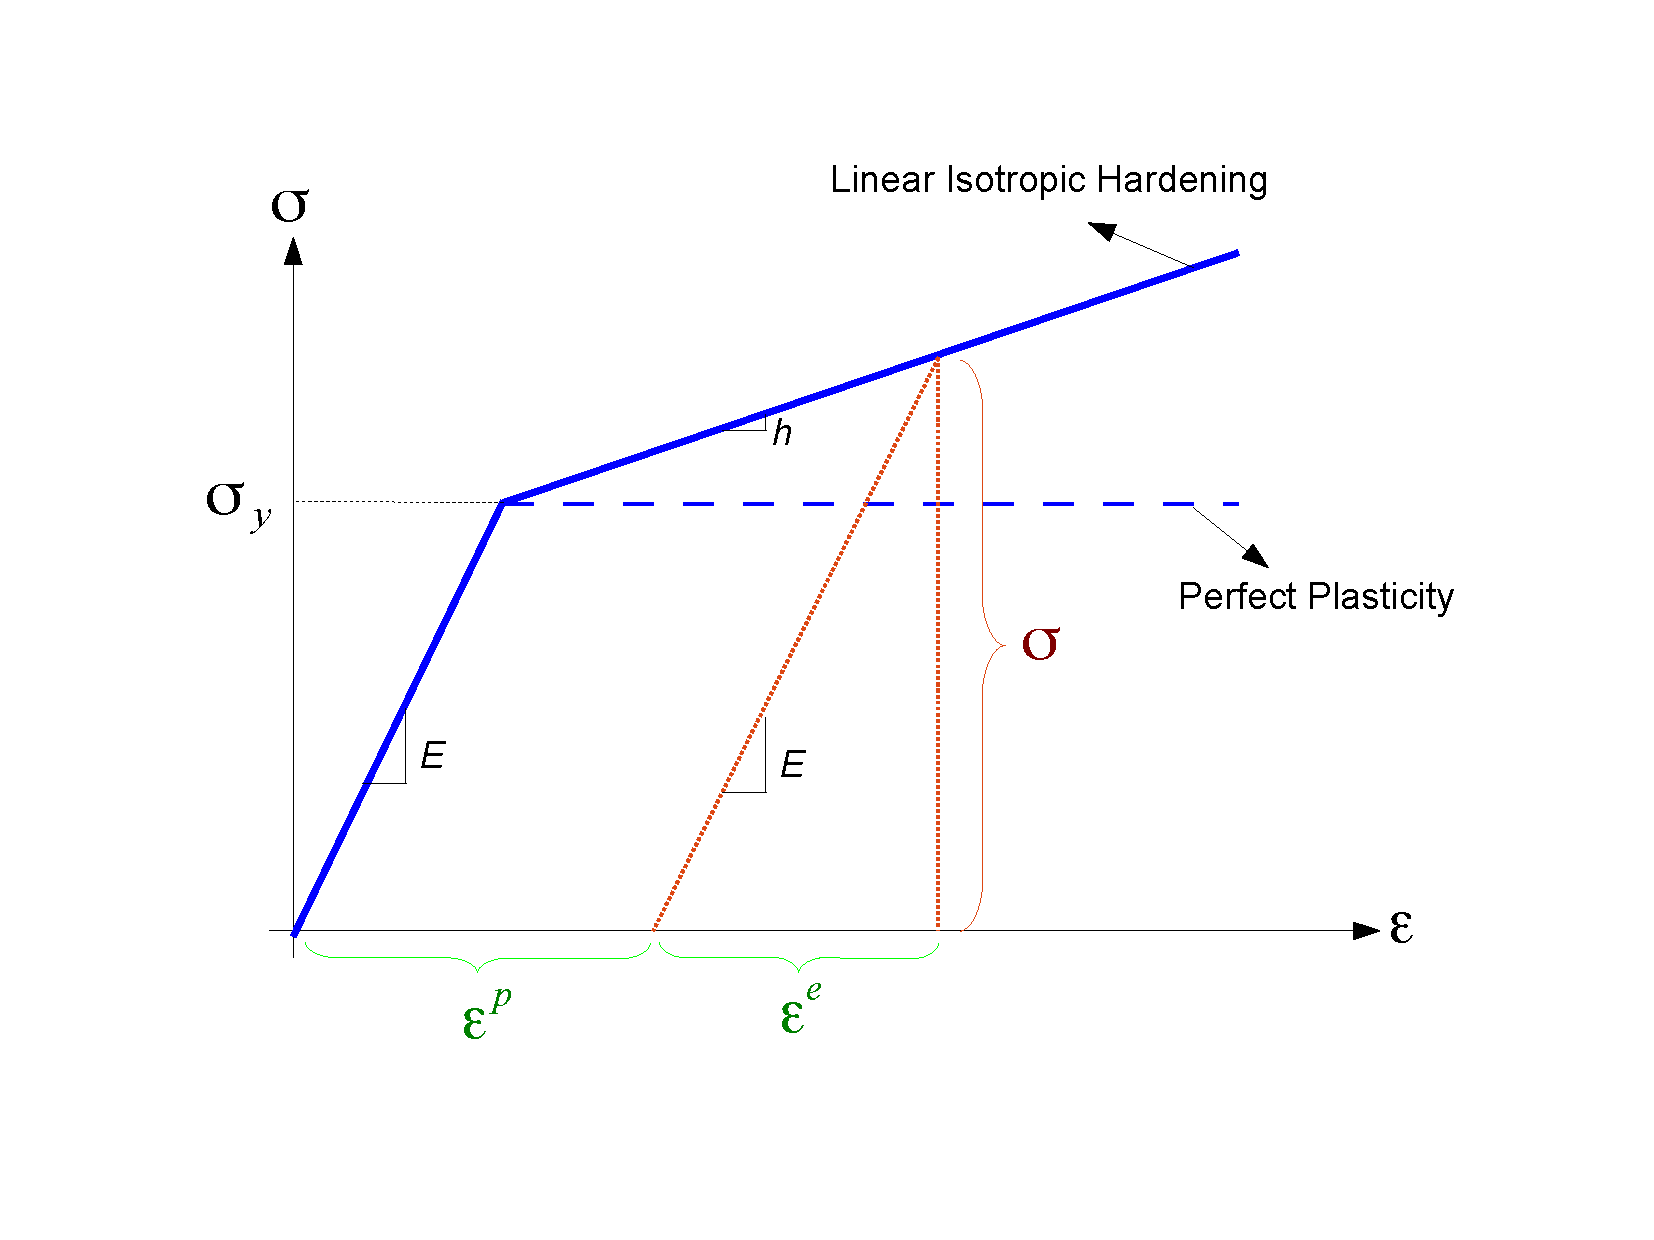
\includegraphics[scale=0.4, clip]{figures/isotropic_hardening_plasticity.pdf}}
   \caption{
    Stress-strain curve for the small-deformation plasticity with a linear isotropic hardening.
   }
  \label{fig:Lin-strain-hard}
\end{figure}

\noindent In this class, the von Mises yield criterion is used. In the von Mises yield criterion, the yield is independent of the hydrostatic stress. Other yielding criteria such as Tresca and Gurson can be easily implemented in this class as well.

In the von Mises yield criterion, the hydrostatic stresses have no effect on the plasticity and consequently the yielding occurs when a critical elastic shear energy is achieved.

\begin{equation} \label{von Mises}
	f = \sigma_{eff} - \sigma_y = (\frac{3}{2} {\mat{\sigma}}^{tr} : {\mat{\sigma}}^{tr})^{1/2}-\sigma_y (\mat{\varepsilon}^p)
\end{equation}

\begin{equation} \label{Hooks law}
 	f < 0 \   \  Elastic \  \ deformation, \                                   \
	f = 0 \   \  Plastic \  \ deformation
\end{equation}

where $\sigma_y$ is the yield strength of the material which can be function of plastic strain in case of hardening type of materials and ${\mat{\sigma}}^{tr}$ is the deviatoric part of stress given by

\begin{equation} \label{deviatoric stress}
	{\mat{\sigma}}^{tr}=\mat{\sigma} - \frac{1}{3} trace(\mat{\sigma}) \mat {I}
\end{equation} 

After yielding $(f = 0)$, normality hypothesis of plasticity determines the direction of plastic flow which is normal to the tangent to the yielding surface at the load point. Then, the tensorial form of the plastic constitutive equation using von Mises yielding criteria (see equation 4.34) may be written as

\begin{equation} \label{plastic contitutive equation}
	\Delta {\mat{\varepsilon}}^p = \Delta p \frac {\partial{f}}{\partial{\mat \sigma}}=\frac{3}{2} \Delta p \frac{{\mat{\sigma}}^{tr}}{\sigma_{eff}}
\end{equation}

In these expressions, the direction of the plastic strain increment (or equivalently,plastic strain rate) is given by $\frac{{\mat{\sigma}}^{tr}}{\sigma_{eff}}$ while the magnitude is defined by the plastic multiplier $\Delta p$. This can be obtained using the \textit{consistency condition} which impose the requirement for the load point to remain on the yielding surface in the plastic regime.

\begin{table}[h]
\centering
  \begin{tabular}{| c | l | c |}
    \hline
    1 & Compute the trial stress & ${\mat{\sigma}}^{tr} = {\mat{\sigma}}_t + 2G\Delta \mat{\varepsilon} + \lambda trace(\Delta \mat{\varepsilon})\mat{I}$ \\[2ex] \hline
    2 & Check the Yielding criteria & $f = (\frac{3}{2} {\mat{\sigma}}^{tr} : {\mat{\sigma}}^{tr})^{1/2}-\sigma_y (\mat{\varepsilon}^p)$ \\[2ex] \hline
    3 & Compute the Plastic multiplier & \begin{tabular}{@{}c@{}c@{}} $d \Delta p = \frac{\sigma^{tr}_{eff} - 3G \Delta P^{(k)}- \sigma_y^{(k)}}{3G + h}		
$ \\ $\Delta p^{(k+1)}=\Delta p^{(k)}+ d\Delta p$ \\$\sigma_y^{(k+1)}=(\sigma_y)_t+ h\Delta p$ \end{tabular}\\ [2ex] \hline
    4 & Compute the plastic strain increment & $\Delta {\mat{\varepsilon}}^p = \frac{3}{2} \Delta p \frac{{\mat{\sigma}}^{tr}}{\sigma_{eff}}$ \\[2ex] \hline
    5 & Compute the stress increment & ${\Delta \mat{\sigma}} = 2G(\Delta \mat{\varepsilon}-\Delta \mat{\varepsilon}^p) + \lambda  trace(\Delta \mat{\varepsilon}-\Delta \mat{\varepsilon}^p)\mat{I}$ \\[2ex] \hline
    6 & update the variables & \begin{tabular}{@{}c@{}} ${\mat{\varepsilon^p}}={\mat{\varepsilon}}^p_t+{\Delta {\mat{\varepsilon}}^p}$ \\    ${\mat{\sigma}}={\mat{\sigma}}_t+{\Delta \mat{\sigma}}$ \end{tabular}\\ [2ex] \hline     
    
  \end{tabular}
  \caption{Summary of the implementation procedure of small-deformation plasticity with linear isotropic hardening in \akantu}
  \label{table:name}
\end{table}


Here, we summarize the implementation procedures for the
small-deformation plasticity with linear isotropic hardening. We use
an implicit integration technique called \textit{the radial return
  method} to obtain the plastic multiplier. This method has an
advantage of being unconditionally stable, however, the accuracy
remains dependent on the step size. The plastic parameters to indicate
in the material file are: \code{$\sigma_y$} (Yield stress) and
\code{h} (Hardening modulus). In addition, the elastic parameters need
to be defined as previous mentioned: \code{E} (Young's modulus),
\code{nu} (Poisson's ratio).


\subsection{Visco-elastic}

% Standard Solid rheological model, see [] J.C. Simo, T.J.R. Hughes,
% "Computational Inelasticity", Springer (1998), see Sections 10.2 and 10.3
Visco-elasticity is characterized by time dependent strain
behavior. Moreover, when such a material undergoes a deformation it
dissipates some energy. This dissipation results in a hysteresis loop
in the stress-strain curve at every loading cycle (see
Figure~\ref{fig:smm:cl:visco-elastic:hyst}). In principle, it can be
applied to many materials, since all materials exhibit a visco-elastic
behavior if subjected to particular conditions (such as high
temperatures).
\begin{figure}[!htb]
  \begin{center}

    \subfloat[]{
      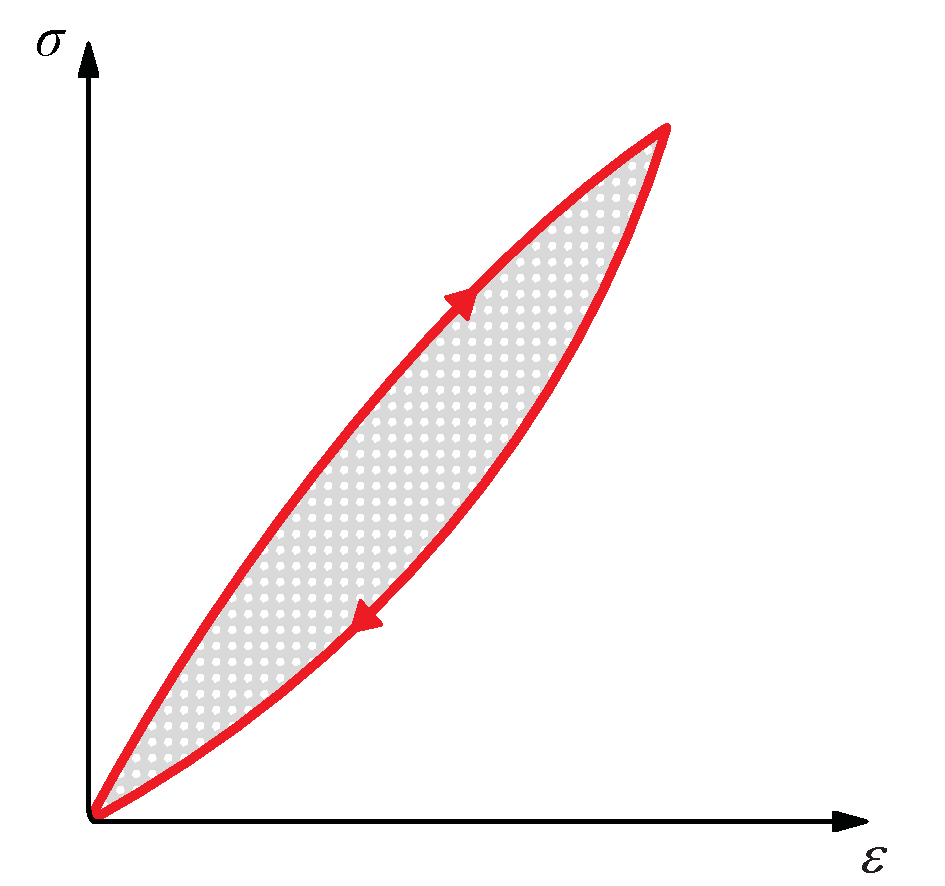
\includegraphics[width=0.4\textwidth,keepaspectratio=true]{figures/stress_strain_visco.pdf}
      \label{fig:smm:cl:visco-elastic:hyst}
    }
    \hspace{0.05\textwidth}
    \subfloat[]{
      \raisebox{0.025\textwidth}{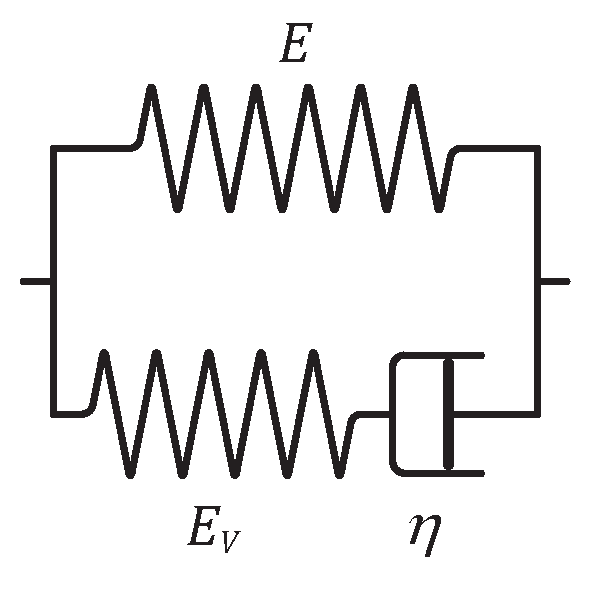
\includegraphics[width=0.3\textwidth,keepaspectratio=true]{figures/visco_elastic_law.pdf}}
      \label{fig:smm:cl:visco-elastic:model}
    }
    \caption{(a) Characteristic stress-strain behavior of a visco-elastic material with hysteresis loop and (b) schematic representation of the standard rheological linear solid visco-elastic model.}
    \label{fig:smm:cl:visco-elastic}
  \end{center}
\end{figure}
The standard rheological linear solid model (see Sections 10.2 and 10.3
of~\cite{simo92}) has been implemented in \akantu. This model results from the
combination of a spring mounted in parallel with a spring and a dashpot
connected in series, as illustrated in
Figure~\ref{fig:smm:cl:visco-elastic:model}. The advantage of this model is that
it allows to account for creep and stress relaxation. The equation that relates
the stress to the strain is (in 1D):
\begin{equation}
  \frac{d\epsilon(t)}{dt} = \left ( E + E_V \right ) ^ {-1} \cdot \left [ \frac{d\sigma(t)}{dt} + \frac{E_V}{\eta}\sigma(t) - \frac{EE_V}{\eta}\epsilon(t) \right ]
\end{equation}
where $\eta$ is the viscosity. The equilibrium condition is unique and is
attained in the limit, as $t \to \infty $. At this stage, the response is
elastic and depends on the Young's modulus $E$.  The parameters requested in the
material file are the following: \code{rho} (density), \code{E} (Young's
modulus), \code{nu} (Poisson's ratio), \code{Plane\_Stress} (if set to zero
plane strain, otherwise plane stress), \code{eta} (dashpot viscosity) and
\code{Ev} (stiffness of the viscous element).

\subsection{Damage}

In the  simplified case of a  linear elastic and brittle  material, isotropic
damage can be represented by a scalar variable $d$, which varies from $0$ to $1$
for  no  damage  to  fully  broken  material  respectively.  The  stress-strain
relationship then becomes:
\begin{equation*}
  \mat{\sigma} = (1-d)\, \mat{C}:\mat{\varepsilon}
\end{equation*}

where  $\mat{\sigma}$,  $\mat{\varepsilon}$ are  the  Cauchy  stress and  strain
tensors, and $\mat{C}$ is the elastic stiffness tensor. This formulation relies
on the definition of a evolution law for the damage variable. In \akantu many
possibilities exists and they are listed below.

\subsubsection{Marigo}
This damage evolution law is energy based as defined by Marigo \cite{marigo81a,
  lemaitre96a}. It is an isotropic damage law.
\begin{align}
  Y &= \frac{1}{2}\mat{\varepsilon}:\mat{C}:\mat{\varepsilon}\\
  F &= Y - Y_d - S d\\
  d &= \left\{
    \begin{array}{l l}
      \mathrm{min}\left(\frac{Y-Y_d}{S},\;1\right) & \mathrm{if}\; F > 0\\
      \mathrm{unchanged} & \mathrm{otherwise}
    \end{array}
  \right.
\end{align}
In this formulation $Y$ is the strain  energy release rate, $Y_d$ is the rupture
criterion and  $S$ is the damage  energy.  The non-local version  of this damage
evolution law is constructed by averaging the energy $Y$.

\subsubsection{Mazars}
This law introduced by Mazars \cite{mazars84a}. It is a behavioral model to
represent damage evolution in concrete. The governing variable in this damage
law is the equivalent strain $\varepsilon_{\st{eq}} =
\sqrt{<\mat{\varepsilon}>_+:<\mat{\varepsilon}>_+}$, with $<.>_+$ the positive
part of the tensor.
The damage the is defined as:
\begin{align}
  D &= \alpha_t^\beta D_t + (1-\alpha_t)^\beta D_c\\
  D_t &= 1 - \frac{\kappa_0 (1- A_t)}{\varepsilon_{\st{eq}}} - A_t \exp^{-B_t(\varepsilon_{\st{eq}}-\kappa_0)}\\
  D_c &= 1 - \frac{\kappa_0 (1- A_c)}{\varepsilon_{\st{eq}}} - A_c
  \exp^{-B_c(\varepsilon_{\st{eq}}-\kappa_0)}\\
  \alpha_t &= \frac{\sum_{i=1}^3<\varepsilon_i>_+\varepsilon_{\st{nd}\;i}}{\varepsilon_{\st{eq}}^2}
\end{align}
With $\kappa_0$ the damage threshold, $A_t$ and $B_t$ the damage parameter in
traction, $A_c$ and $B_c$ the damage parameter in compression, $\beta$ is the
shear parameter. $\alpha_t$ is the coupling parameter between traction and
compression, the $\varepsilon_i$ are the eigenstrain and the
$\varepsilon_{\st{nd}\;i}$ are the eigen value of the strain if the material
would be sound.

The coefficient $A$ and $B$ are the post-pic asymptotic
value and the decay shape parameters.

%%% Local Variables: 
%%% mode: latex
%%% TeX-master: "manual"
%%% End: 
